\documentclass[10pt]{article}
\usepackage[hmargin=1.25cm, vmargin=1.5cm]{geometry}
\usepackage{bbding}
\usepackage{multirow}
\usepackage{amssymb}
\usepackage{eurosym}
\usepackage{color,graphicx}
\usepackage[usenames,dvipsnames]{xcolor}
\usepackage{fontspec,xltxtra,xunicode}
\defaultfontfeatures{Mapping=tex-text}
\setromanfont[Mapping=tex-text]{Hoefler Text}
\setsansfont[Scale=MatchLowercase,Mapping=tex-text]{Gill Sans}
\setmonofont[Scale=MatchLowercase]{Andale Mono}
\DeclareGraphicsExtensions{.pdf,.png,.jpg}
%Setup hyperref package, and colours for links, text and headings
\usepackage{hyperref}
%\definecolor{linkcolor}
%{HTML}{FF0080} %light purple link for the email
\definecolor{linkcolor}{HTML}{00008B}
\definecolor{shade}{HTML}{D4D7FE}      %light blue shade
%\definecolor{text1}{HTML}{2b2b2b}      %text is almost black
\definecolor{text1}{HTML}{000000}      %text is black
\definecolor{headings}{HTML}{00008B}   %navy blue
\hypersetup{   colorlinks,breaklinks,
               urlcolor=linkcolor,
               linkcolor=linkcolor
}

\usepackage{fancyhdr}                  %custom footer
\pagestyle{fancy}
\fancyhf{}
\rfoot{\small\color{headings} {\sffamily Last update: \today}.
Typeset with X\LaTeX}
\renewcommand{\headrulewidth}{0pt}

\usepackage{titlesec}                  %custom \section

\titleformat{\section}
   {\color{headings}
      \scshape\Large\raggedright}{}{0em}{}[\color{black}\titlerule]

\titlespacing{\section}{0pt}{0pt}{3pt}

\begin{document}
\color{text1} % set text color for the whole doc
     \par{\centering{\sffamily\huge J. Randall Hunt}\\
      \color{headings}\fontspec[Variant = 2]{Zapfino} Resumé \par
      %\color{headings}\fontspec[Variant = 2]
      %{Zapfino}R\'esum\'e\\[20pt]
      {\color{white} \hrule}} %does this rule really change anything?

\begin{minipage}[t]{0.5\textwidth}

\vspace{0pt}   %trick

\section{Work Experience}

   \raggedleft
   \textsc{\normalsize June 2012 -- Present}\par
   \raggedright\large Python Engineer\\
   \textsc{\href{http://mongodb.org/}{The MongoDB Company}}\\
   \normalsize{Managed continuous integration (buildbot, jenkins, travis)
   across multiple platforms (FreeBSD, Windows, Linux, OSX). Substantially
   reduced cost of maintaining buildslaves (\$10000s per month). Attended
   confrences and gave technical presenations on devops, mongodb, and
   python. Contributed to several open-source projects.}\\[5pt]
   \raggedleft
   \textsc{\normalsize May 2011 -- Oct 2011}\par
   \raggedright\large Python Engineer\\
   \textsc{hackNY, \href{http://fondu.com/}{Fondu}}\\
   \normalsize{Designed and implemented a collaborative filtering
   recommendation engine in Python and C which improved recommendation
   speed (initial response and pre-calculations) by 800\%. Used SciPy,
   NumPy, and Weave to accheive these dramatic speed improvements. Also
   wrote scripts to automate deployment and logging on Amazon Web Services
   }\\[5pt]

   \raggedleft
   \textsc{\normalsize January 2011 -- May 2011}\par
   \raggedright\large Undergraduate Researcher\\
   \textsc{NASA Ames Research Center}\\
   \normalsize{Created an Automatic KML Tour Generator and KML Tour
   Editor using Django, Python, SQL, and Javascript. Media import tool
   pulls from several different sources and loads all data into a
   database. Project generated a whole new set of data products for
   the Maps team.}\\[5pt]

   \raggedleft
   \textsc{\normalsize June 2010 -- August 2010}\par
   \raggedright\large Undergraduate Researcher\\
   \textsc{NASA Langley Research Center}\\
   \normalsize{Worked on several tools for mass properties evaluation
   which culminated in the design a mass properties API. Also worked
   with an 8 person team to design and evaluate a series of tests on
   a flotation concept. If implemented project could save millons of
   dollars. Findings were published to NASA's main webpage, AIAA
   newsletter, and several other notable websites.}\\[5pt]

\section{\textsc{Technical Skills}}
   \begin{tabular}{rl}
      \textbf{\textsc{Languages}}:
                        & \textbf{Professional}:\\
                        & c, java, python\\
                        & HTML/CSS/javascript\\
                        & \textbf{Familiar}:\\
                        & ruby, go, prolog, php, C++\\
                        & perl, Objective-C, LISP\\
                        & \\
      \textbf{\textsc{Tools and Frameworks}}:
                        & general devops, chef, puppet\\
                        & mongodb, sql, vim, emacs, git\\
                        & \\
      \textbf{\textsc{Mathematics}}:
                        & Formal Logic and Proof Techniques,\\
                        & Linear Algebra, Calculus,\\
                        & Statistics, Discrete Structures\\
\end{tabular}
\end{minipage}
\hfill
\begin{minipage}[t]{0.44\textwidth}

   \vspace{-10pt} %trick for alignment
\colorbox{shade}{\textcolor{text1}{
      \begin{tabular}{c|p{4.25cm}r}
                                    %Can't include this in a lot of forms.
                                    %& Born in North Carolina in 1991\\
         \raisebox{-1pt}{\Phone}    &+1(910) 249-9253
         &\raisebox{2.9pt}{\multirow{2}{*}{
             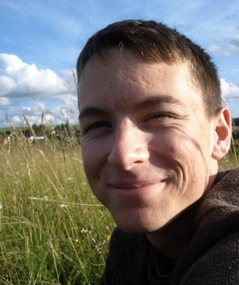
\includegraphics[height=1.45cm]{randall}
             }}\\
         \raisebox{-1pt}{\textsc{www}} &
         \href{http://blog.ranman.org/}{www.ranman.org}&\\
         \raisebox{-3pt}{\Envelope} &
         \href{mailto:randallhunt@gmail.com}{randall.hunt@gmail.com}&
      \end{tabular}
    }
}\\[3pt]

\section{Education}
\begin{tabular}{rl}
      & \textbf{Western Carolina University}\\
      & Cullowhee, NC\\
      &\\
      & \textbf{Punahou}\\
      & Honolulu, Hawaii\\
      &\\
      & \textbf{Université Catholique De L'Ouest}\\
      & Angers, France\\
\end{tabular}\\[5pt]

\section{Languages}
\begin{tabular}{rl}
   \textsc{French}   &  Proficient\\
   \textsc{German}   &  Conversational\\
   \textsc{Spanish}  &  Learner\\
\end{tabular}\\[5pt]

\section{Relevant Projects (available on github)}
   Gitshots in Python\\
   Multiuser Chat System in Java\\
   Address Book with RMI in Java\\
   Set Associative Cache Simulator in Java\\
   Paint Clone in Java\\
   Email Client in Java\\
   Tokenizer and Parser in C\\
   Wireless Sensor Grapher in TinyC+Java\\
   TCP Implementation in TinyC\\
   Adventure Game in Prolog\\

\section{Awards/Presentations/Stuff}
   \href{http://hackny.org/a/about/}{HackNY Fellow and Mentor}
   IEEE Member\\
   \href{http://polaris.cs.wcu.edu/~acm/}{Student ACM Chapter}\\
   \href{https://github.com/ranman}{Open-Source Contributor}\\
   Active on \href{http://stackoverflow.com/users/240004/ranman}
   {StackOverflow}\\
   Passionate about Robotics\href{http://robotics.punahou.edu/}{[1]}
   \href{http://irg.arc.nasa.gov}{[2]}\\
   \href{http://www.youtube.com/user/ranman96734}{Rubik's Cubes}\\
   Bicycles!
   Academic Technology Advisory Committee\\
   AP Scholar's Award\\
   Several Presenations at NASA\\
   Honors College\\
   Won several hackathons\\
\end{minipage}
\end{document}
